\documentclass[12pt]{article}
\usepackage{geometry}
\geometry{margin=0.9in}
\usepackage{tikz}
\usepackage{enumitem}
\usepackage{parskip}
\usepackage{xcolor}
\definecolor{isaorange}{HTML}{C2410C}

\newcommand{\bigtask}[1]{\par\medskip\noindent{\large\textbf{\color{isaorange}#1}}\par}

% A box with a dashed line down the middle, for "draw half, then complete it".
\newcommand{\mirrorbox}[1]{%
  \par\vspace{4pt}\noindent
  \begin{tikzpicture}
    \draw[rounded corners, line width=1pt] (0,0) rectangle (\linewidth,#1);
    \draw[dashed, gray, line width=1pt] (0.5\linewidth,0) -- (0.5\linewidth,#1);
    \node[gray] at (0.5\linewidth, -0.35) {\footnotesize fold line};
  \end{tikzpicture}\par\vspace{10pt}}

\begin{document}

\begin{center}
  {\huge\textbf{Mirror Magic}}\\[2pt]
  {\large Folds where both halves match}
\end{center}
\vspace{0.3cm}

\bigtask{1. Draw half, then complete it}
Draw half of a butterfly on the left of the dashed line. Then draw the matching
half on the right so the two sides match.
\mirrorbox{5cm}

\bigtask{2. Which letters does a mirror complete?}
Circle the letters that have a matching left and right half:
\begin{center}
  {\Huge A \quad R \quad M \quad F \quad T \quad W \quad G \quad H}
\end{center}

\bigtask{3. Fold and cut}
\begin{enumerate}[leftmargin=*]
  \item Fold a paper in half. Cut half a heart on the fold. Open it.
  \item Fold a circle of paper into a skinny wedge. Snip the edges. Open it
        slowly to find a snowflake.
\end{enumerate}
How many matching points does your snowflake have? \underline{\hspace{3cm}}

\bigtask{4. How many fold lines does a square have?}
Fold a square of paper different ways. Draw every fold line you find on this
square:
\begin{center}
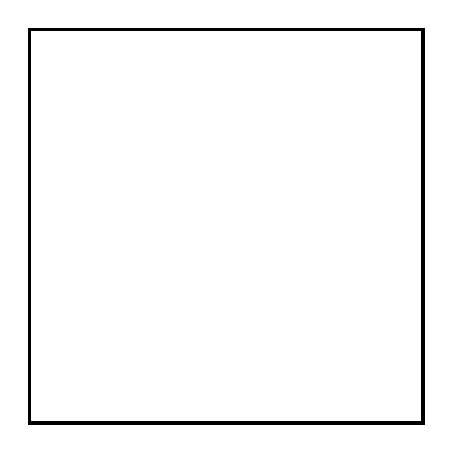
\begin{tikzpicture}
  \draw[line width=1.2pt] (0,0) rectangle (5,5);
\end{tikzpicture}
\end{center}
I found \underline{\hspace{2cm}} fold lines.

\bigtask{5. Symmetry hunt}
Find five things in the room with a line of symmetry. Draw or write them:
\begin{enumerate}[leftmargin=*, itemsep=10pt]
  \item \hrulefill
  \item \hrulefill
  \item \hrulefill
  \item \hrulefill
  \item \hrulefill
\end{enumerate}

\end{document}
